\documentclass[12pt,a4paper]{article}
\usepackage[utf8]{inputenc}
\usepackage[english]{babel}
\usepackage[T1]{fontenc}
\usepackage[margin=2.5cm]{geometry}
\usepackage{hyperref}
\usepackage{tabularx}
\usepackage{booktabs}
\usepackage{xcolor}
\usepackage{graphicx}

\title{\vspace{-2cm}\textbf{BoosterChallenge VUT 2026 -- Project Proposal}}
\author{}
\date{}

\begin{document}

\maketitle
\vspace{-1.5cm}


\tableofcontents

\vspace{1cm}

\section{Project Name and Team}

\subsection*{Project Identifier}
SyncUp

\subsection*{Project Description}
A user-friendly cross-platform appointment scheduling system designed to simplify booking meetings between students and professors. It provides role-based interfaces to ensure quick scheduling for students and efficient management for professors.

\subsection*{Team}
Names of the core team members and their emails. 

\vspace{0.5cm}
\begin{center}
\renewcommand{\arraystretch}{1.5}
\begin{tabularx}{\textwidth}{|X|X|X|}
\hline
\textbf{Name and Surname} & \textbf{Email (Primary)} & \textbf{Faculty} \\
\hline
Adar Otieno & xotiena00@vutbr.cz & FIT VUT \\
\hline
Eyobed Awel Nuri & xnuriey00@vutbr.cz & FIT VUT \\
\hline
Pengwei Jiang & xjiangp00@vutbr.cz & FIT VUT \\
\hline
Mengran Zhao & xzhaome00@vutbr.cz & FIT VUT \\
\hline
\end{tabularx}
\end{center}

\vspace{0.2cm}
\noindent
\textit{Note: The project team consists of international students and our primary language of communication is English.}
\section{Product}

\subsection{Target Product}
A cross-platform application (desktop and mobile) featuring a calendar-based interface, minimal booking flow, and support for light/dark modes. It includes a clear separation between student and professor roles. Students have an interface optimized for speed and clarity in booking, while professors are equipped with tools for controlling, overviewing, and bulk-managing multiple appointments. Additionally, the system will integrate our dedicated indoor mapping solution to provide seamless door-to-door navigation for scheduled appointments. 

\subsection{Benefit}
Currently, scheduling academic appointments often relies on inefficient email communication. Our system benefits both students and professors by saving time, reducing miscommunication, and providing a centralized overview of consultations. It directly addresses a common and practical issue in academic environments based on real user needs.

\section{Product Development}

\subsection{Current State of the Project}
The project currently has a working MVP that is deployed and accessible. The frontend-backend integration using Flutter and PocketBase is fully synchronized, handling availability, booking, cancellation, and user data. Initial usability and interaction flow testing have been conducted.

\begin{figure}[h]
    \centering
    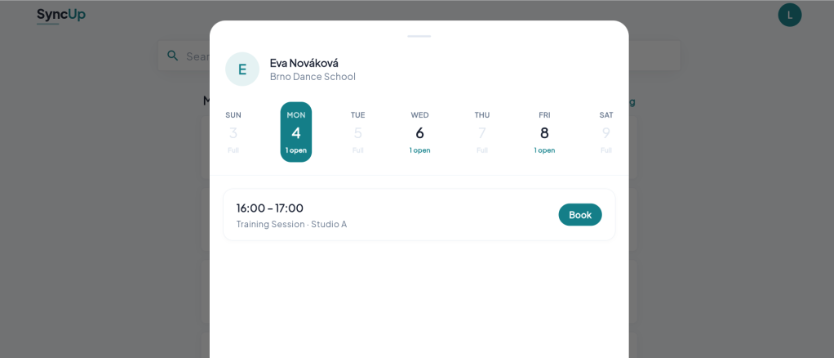
\includegraphics[width=0.9\textwidth]{Screenshot.png}
    \caption{SyncUp MVP User Interface}
\end{figure}

\subsection{Target State within the Competition}
During the competition (June--August), we will focus on:
\begin{itemize}
    \item \textbf{Indoor Mapping Integration:} Integrating door-to-door routing for scheduled appointments.
    \item \textbf{Advanced Scheduling:} Implementing complex booking constraints and integrating directly with university calendars (e.g., IS VUT).
    \item \textbf{Validation:} Scaling our user testing phase to gather feedback.
\end{itemize}

\subsection{Technology}
\begin{itemize}
    \item \textbf{Frontend:} Flutter (cross-platform framework for desktop and mobile)
    \item \textbf{Backend:} PocketBase (lightweight backend solution)
    \item \textbf{Design \& Prototyping:} Figma
\end{itemize}

\section{Optional}

\subsection{Link to Study}
As students, we directly experienced the inefficiencies of email-based scheduling, which motivated this project. The system design and evaluation leverage our academic knowledge in UI/UX(course UXI) and software engineering.
\subsection{Financial Plan}
Estimated costs for MVP deployment include server hosting for the PocketBase backend (approx. \$5--\$10/month). Future publishing would require an Apple Developer account (\$99/year) and Google Play Console access (\$25 one-time fee).

\end{document}
